% Options for packages loaded elsewhere
\PassOptionsToPackage{unicode}{hyperref}
\PassOptionsToPackage{hyphens}{url}
\PassOptionsToPackage{dvipsnames,svgnames,x11names}{xcolor}
%
\documentclass[
  letterpaper,
  DIV=11,
  numbers=noendperiod]{scrreprt}

\usepackage{amsmath,amssymb}
\usepackage{iftex}
\ifPDFTeX
  \usepackage[T1]{fontenc}
  \usepackage[utf8]{inputenc}
  \usepackage{textcomp} % provide euro and other symbols
\else % if luatex or xetex
  \usepackage{unicode-math}
  \defaultfontfeatures{Scale=MatchLowercase}
  \defaultfontfeatures[\rmfamily]{Ligatures=TeX,Scale=1}
\fi
\usepackage{lmodern}
\ifPDFTeX\else  
    % xetex/luatex font selection
\fi
% Use upquote if available, for straight quotes in verbatim environments
\IfFileExists{upquote.sty}{\usepackage{upquote}}{}
\IfFileExists{microtype.sty}{% use microtype if available
  \usepackage[]{microtype}
  \UseMicrotypeSet[protrusion]{basicmath} % disable protrusion for tt fonts
}{}
\makeatletter
\@ifundefined{KOMAClassName}{% if non-KOMA class
  \IfFileExists{parskip.sty}{%
    \usepackage{parskip}
  }{% else
    \setlength{\parindent}{0pt}
    \setlength{\parskip}{6pt plus 2pt minus 1pt}}
}{% if KOMA class
  \KOMAoptions{parskip=half}}
\makeatother
\usepackage{xcolor}
\setlength{\emergencystretch}{3em} % prevent overfull lines
\setcounter{secnumdepth}{5}
% Make \paragraph and \subparagraph free-standing
\ifx\paragraph\undefined\else
  \let\oldparagraph\paragraph
  \renewcommand{\paragraph}[1]{\oldparagraph{#1}\mbox{}}
\fi
\ifx\subparagraph\undefined\else
  \let\oldsubparagraph\subparagraph
  \renewcommand{\subparagraph}[1]{\oldsubparagraph{#1}\mbox{}}
\fi

\usepackage{color}
\usepackage{fancyvrb}
\newcommand{\VerbBar}{|}
\newcommand{\VERB}{\Verb[commandchars=\\\{\}]}
\DefineVerbatimEnvironment{Highlighting}{Verbatim}{commandchars=\\\{\}}
% Add ',fontsize=\small' for more characters per line
\usepackage{framed}
\definecolor{shadecolor}{RGB}{241,243,245}
\newenvironment{Shaded}{\begin{snugshade}}{\end{snugshade}}
\newcommand{\AlertTok}[1]{\textcolor[rgb]{0.68,0.00,0.00}{#1}}
\newcommand{\AnnotationTok}[1]{\textcolor[rgb]{0.37,0.37,0.37}{#1}}
\newcommand{\AttributeTok}[1]{\textcolor[rgb]{0.40,0.45,0.13}{#1}}
\newcommand{\BaseNTok}[1]{\textcolor[rgb]{0.68,0.00,0.00}{#1}}
\newcommand{\BuiltInTok}[1]{\textcolor[rgb]{0.00,0.23,0.31}{#1}}
\newcommand{\CharTok}[1]{\textcolor[rgb]{0.13,0.47,0.30}{#1}}
\newcommand{\CommentTok}[1]{\textcolor[rgb]{0.37,0.37,0.37}{#1}}
\newcommand{\CommentVarTok}[1]{\textcolor[rgb]{0.37,0.37,0.37}{\textit{#1}}}
\newcommand{\ConstantTok}[1]{\textcolor[rgb]{0.56,0.35,0.01}{#1}}
\newcommand{\ControlFlowTok}[1]{\textcolor[rgb]{0.00,0.23,0.31}{#1}}
\newcommand{\DataTypeTok}[1]{\textcolor[rgb]{0.68,0.00,0.00}{#1}}
\newcommand{\DecValTok}[1]{\textcolor[rgb]{0.68,0.00,0.00}{#1}}
\newcommand{\DocumentationTok}[1]{\textcolor[rgb]{0.37,0.37,0.37}{\textit{#1}}}
\newcommand{\ErrorTok}[1]{\textcolor[rgb]{0.68,0.00,0.00}{#1}}
\newcommand{\ExtensionTok}[1]{\textcolor[rgb]{0.00,0.23,0.31}{#1}}
\newcommand{\FloatTok}[1]{\textcolor[rgb]{0.68,0.00,0.00}{#1}}
\newcommand{\FunctionTok}[1]{\textcolor[rgb]{0.28,0.35,0.67}{#1}}
\newcommand{\ImportTok}[1]{\textcolor[rgb]{0.00,0.46,0.62}{#1}}
\newcommand{\InformationTok}[1]{\textcolor[rgb]{0.37,0.37,0.37}{#1}}
\newcommand{\KeywordTok}[1]{\textcolor[rgb]{0.00,0.23,0.31}{#1}}
\newcommand{\NormalTok}[1]{\textcolor[rgb]{0.00,0.23,0.31}{#1}}
\newcommand{\OperatorTok}[1]{\textcolor[rgb]{0.37,0.37,0.37}{#1}}
\newcommand{\OtherTok}[1]{\textcolor[rgb]{0.00,0.23,0.31}{#1}}
\newcommand{\PreprocessorTok}[1]{\textcolor[rgb]{0.68,0.00,0.00}{#1}}
\newcommand{\RegionMarkerTok}[1]{\textcolor[rgb]{0.00,0.23,0.31}{#1}}
\newcommand{\SpecialCharTok}[1]{\textcolor[rgb]{0.37,0.37,0.37}{#1}}
\newcommand{\SpecialStringTok}[1]{\textcolor[rgb]{0.13,0.47,0.30}{#1}}
\newcommand{\StringTok}[1]{\textcolor[rgb]{0.13,0.47,0.30}{#1}}
\newcommand{\VariableTok}[1]{\textcolor[rgb]{0.07,0.07,0.07}{#1}}
\newcommand{\VerbatimStringTok}[1]{\textcolor[rgb]{0.13,0.47,0.30}{#1}}
\newcommand{\WarningTok}[1]{\textcolor[rgb]{0.37,0.37,0.37}{\textit{#1}}}

\providecommand{\tightlist}{%
  \setlength{\itemsep}{0pt}\setlength{\parskip}{0pt}}\usepackage{longtable,booktabs,array}
\usepackage{calc} % for calculating minipage widths
% Correct order of tables after \paragraph or \subparagraph
\usepackage{etoolbox}
\makeatletter
\patchcmd\longtable{\par}{\if@noskipsec\mbox{}\fi\par}{}{}
\makeatother
% Allow footnotes in longtable head/foot
\IfFileExists{footnotehyper.sty}{\usepackage{footnotehyper}}{\usepackage{footnote}}
\makesavenoteenv{longtable}
\usepackage{graphicx}
\makeatletter
\def\maxwidth{\ifdim\Gin@nat@width>\linewidth\linewidth\else\Gin@nat@width\fi}
\def\maxheight{\ifdim\Gin@nat@height>\textheight\textheight\else\Gin@nat@height\fi}
\makeatother
% Scale images if necessary, so that they will not overflow the page
% margins by default, and it is still possible to overwrite the defaults
% using explicit options in \includegraphics[width, height, ...]{}
\setkeys{Gin}{width=\maxwidth,height=\maxheight,keepaspectratio}
% Set default figure placement to htbp
\makeatletter
\def\fps@figure{htbp}
\makeatother
% definitions for citeproc citations
\NewDocumentCommand\citeproctext{}{}
\NewDocumentCommand\citeproc{mm}{%
  \begingroup\def\citeproctext{#2}\cite{#1}\endgroup}
\makeatletter
 % allow citations to break across lines
 \let\@cite@ofmt\@firstofone
 % avoid brackets around text for \cite:
 \def\@biblabel#1{}
 \def\@cite#1#2{{#1\if@tempswa , #2\fi}}
\makeatother
\newlength{\cslhangindent}
\setlength{\cslhangindent}{1.5em}
\newlength{\csllabelwidth}
\setlength{\csllabelwidth}{3em}
\newenvironment{CSLReferences}[2] % #1 hanging-indent, #2 entry-spacing
 {\begin{list}{}{%
  \setlength{\itemindent}{0pt}
  \setlength{\leftmargin}{0pt}
  \setlength{\parsep}{0pt}
  % turn on hanging indent if param 1 is 1
  \ifodd #1
   \setlength{\leftmargin}{\cslhangindent}
   \setlength{\itemindent}{-1\cslhangindent}
  \fi
  % set entry spacing
  \setlength{\itemsep}{#2\baselineskip}}}
 {\end{list}}
\usepackage{calc}
\newcommand{\CSLBlock}[1]{\hfill\break\parbox[t]{\linewidth}{\strut\ignorespaces#1\strut}}
\newcommand{\CSLLeftMargin}[1]{\parbox[t]{\csllabelwidth}{\strut#1\strut}}
\newcommand{\CSLRightInline}[1]{\parbox[t]{\linewidth - \csllabelwidth}{\strut#1\strut}}
\newcommand{\CSLIndent}[1]{\hspace{\cslhangindent}#1}

\KOMAoption{captions}{tableheading}
\makeatletter
\@ifpackageloaded{bookmark}{}{\usepackage{bookmark}}
\makeatother
\makeatletter
\@ifpackageloaded{caption}{}{\usepackage{caption}}
\AtBeginDocument{%
\ifdefined\contentsname
  \renewcommand*\contentsname{Tabla de contenidos}
\else
  \newcommand\contentsname{Tabla de contenidos}
\fi
\ifdefined\listfigurename
  \renewcommand*\listfigurename{Listado de Figuras}
\else
  \newcommand\listfigurename{Listado de Figuras}
\fi
\ifdefined\listtablename
  \renewcommand*\listtablename{Listado de Tablas}
\else
  \newcommand\listtablename{Listado de Tablas}
\fi
\ifdefined\figurename
  \renewcommand*\figurename{Figura}
\else
  \newcommand\figurename{Figura}
\fi
\ifdefined\tablename
  \renewcommand*\tablename{Tabla}
\else
  \newcommand\tablename{Tabla}
\fi
}
\@ifpackageloaded{float}{}{\usepackage{float}}
\floatstyle{ruled}
\@ifundefined{c@chapter}{\newfloat{codelisting}{h}{lop}}{\newfloat{codelisting}{h}{lop}[chapter]}
\floatname{codelisting}{Listado}
\newcommand*\listoflistings{\listof{codelisting}{Listado de Listados}}
\makeatother
\makeatletter
\makeatother
\makeatletter
\@ifpackageloaded{caption}{}{\usepackage{caption}}
\@ifpackageloaded{subcaption}{}{\usepackage{subcaption}}
\makeatother
\makeatletter
\@ifpackageloaded{tikz}{}{\usepackage{tikz}}
\makeatother
        \newcommand*\circled[1]{\tikz[baseline=(char.base)]{
          \node[shape=circle,draw,inner sep=1pt] (char) {{\scriptsize#1}};}}  
                  
\ifLuaTeX
\usepackage[bidi=basic]{babel}
\else
\usepackage[bidi=default]{babel}
\fi
\babelprovide[main,import]{spanish}
% get rid of language-specific shorthands (see #6817):
\let\LanguageShortHands\languageshorthands
\def\languageshorthands#1{}
\ifLuaTeX
  \usepackage{selnolig}  % disable illegal ligatures
\fi
\usepackage{bookmark}

\IfFileExists{xurl.sty}{\usepackage{xurl}}{} % add URL line breaks if available
\urlstyle{same} % disable monospaced font for URLs
\hypersetup{
  pdftitle={Título del trabajo},
  pdfauthor={Nombre y Apellidos},
  pdflang={es},
  colorlinks=true,
  linkcolor={blue},
  filecolor={Maroon},
  citecolor={Blue},
  urlcolor={Blue},
  pdfcreator={LaTeX via pandoc}}

\title{Título del trabajo}
\author{Nombre y Apellidos}
\date{2024-05-27}

\begin{document}
\maketitle

\renewcommand*\contentsname{Tabla de contenidos}
{
\hypersetup{linkcolor=}
\setcounter{tocdepth}{2}
\tableofcontents
}
\bookmarksetup{startatroot}

\chapter{}\label{section}

\bookmarksetup{startatroot}

\chapter{Introducción}\label{sec-introduccion}

\noindent Cualquier capítulo puede tener múltiples apartados, como el
Sección~\ref{sec-lista-de-items} o el Sección~\ref{sec-enumeraciones} de
este mismo capítulo.

También está el Sección~\ref{sec-primera-seccion} del
Capítulo~\ref{sec-capitulo-dos} que tiene la \textbf{?@fig-otra}.

Es buena idea usar \texttt{\textbackslash{}noindent} --que es un comando
de \LaTeX{}-- al principio del primer párrafo, tras el encabezado de una
sección o capítulo, para desactivar la sangría temporalmente.

\section{Listas de elementos}\label{sec-lista-de-items}

\noindent Esta la lista de elementos del
Sección~\ref{sec-lista-de-items}:

\begin{itemize}
\tightlist
\item
  Item 1

  \begin{itemize}
  \tightlist
  \item
    Item 1
  \item
    Item 2
  \item
    Item 3
  \item
    Item 4
  \end{itemize}
\item
  Item 2
\item
  Item 3
\item
  Item 4
\end{itemize}

\section{Enumeraciones}\label{sec-enumeraciones}

\noindent Esto es una lista enumerada, que puede estar relacionada con
la Figura~\ref{fig-introduccion}

\begin{enumerate}
\def\labelenumi{\arabic{enumi}.}
\tightlist
\item
  Item 1

  \begin{enumerate}
  \def\labelenumii{\arabic{enumii}.}
  \tightlist
  \item
    Item 1
  \item
    Item 2
  \item
    Item 3
  \end{enumerate}
\item
  Item 2
\item
  Item 3
\end{enumerate}

\section{Figuras y tablas}\label{figuras-y-tablas}

\noindent En la Figura~\ref{fig-introduccion} se puede ver una figura de
ejemplo. Las figuras --y, opcionalmente, los listados de código-- son
flotantes. Esto quiere decir que \LaTeX{} las intentará ubicar en el
mejor lugar posible al componer el documento, intentando respetar
ciertas reglas tipográficas. Como este lugar puede ser diferente a la
posición que realmente ocupan en el texto, \textbf{es importante
referenciar en el texto todas las figuras}, en los diferentes puntos
donde se hable de ellas.

\begin{figure}[htbp]

\centering{

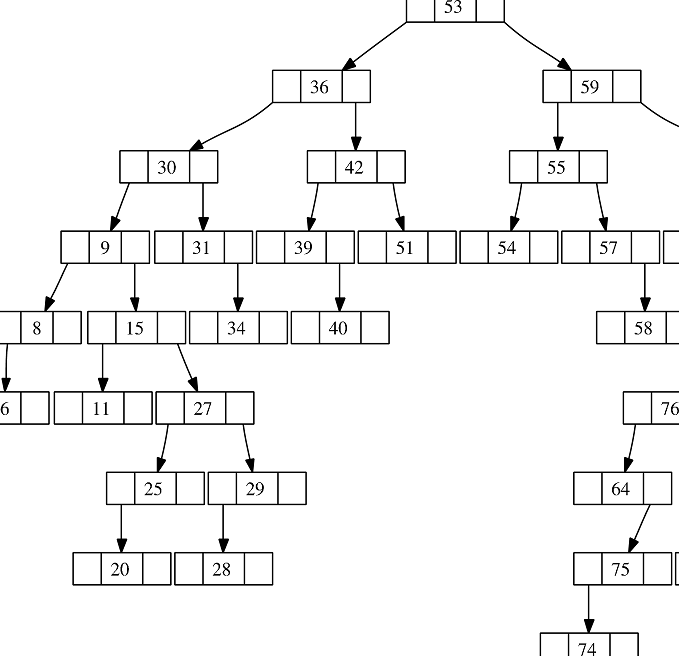
\includegraphics[width=0.8\textwidth,height=\textheight]{images/figura_1.png}

}

\caption{\label{fig-introduccion}Ejemplo de figura.}

\end{figure}%

Por otro lando, la Tabla~\ref{tbl-presupuesto} en el
Capítulo~\ref{sec-presupuesto} es un ejemplo de tabla hecha con
Markdown.

\section{Código y algoritmos}\label{cuxf3digo-y-algoritmos}

\noindent En el Apéndice~\ref{sec-apendice-uno} se pueden observar
varios ejemplos de entornos para describir algoritmos y código.

\section{Citas}\label{citas}

\noindent Las referencias bibliográficas se deben indicar en el archivo
\texttt{referencias.bib} y se citan en el texto. Las referencias no
citadas no aparecerán en el apartado de la bibliografía.

Las citas pueden ser entre paréntesis (Smith, 2021) o \emph{en línea},
como la de Doe (2022).

Las reglas para citar (Universidad de La Laguna, 2023) permiten citar
cualquier cosa: artículos de investigación, libros, entradas de la
Wikipedia, blogs, vídeos de Youtube o repositorios de GitHub, entre
otros.

En el Capítulo~\ref{sec-capitulo-cuatro} se puede ver otro tipo de cita,
donde se traslada de forma literal una porción del texto original al
documento.

\section{Otra sección\ldots{}}\label{otra-secciuxf3n}

\noindent [lipsum {} {]}\{.quarto-shortcode\_\_ data-is-shortcode=``1''
data-raw=``\{\{\textless{} lipsum 1 \textgreater\}\}''\}

\subsection{Con subsección\ldots{}}\label{con-subsecciuxf3n}

\noindent [lipsum {} {]}\{.quarto-shortcode\_\_ data-is-shortcode=``1''
data-raw=``\{\{\textless{} lipsum 2 \textgreater\}\}''\}

\bookmarksetup{startatroot}

\chapter{Título del Capítulo 2}\label{sec-capitulo-dos}

\noindent Los capítulos intermedios sirven para cubrir los siguientes
aspectos: antecedentes, problemática o estado del arte, objetivos, fases
y desarrollo del proyecto.

En el capítulo anterior se ha introducido la
Figura~\ref{fig-introduccion} y en este la \textbf{?@fig-otra}.

\section{Primera sección de otro capítulo}\label{sec-primera-seccion}

\noindent [lipsum {} {]}\{.quarto-shortcode\_\_ data-is-shortcode=``1''
data-raw=``\{\{\textless{} lipsum 3 \textgreater\}\}''\}

\subsection{Primera subsección}\label{primera-subsecciuxf3n}

\noindent [lipsum {} {]}\{.quarto-shortcode\_\_ data-is-shortcode=``1''
data-raw=``\{\{\textless{} lipsum 4 \textgreater\}\}''\}

\subsection{Segunda subsección}\label{segunda-subsecciuxf3n}

\noindent [lipsum {} {]}\{.quarto-shortcode\_\_ data-is-shortcode=``1''
data-raw=``\{\{\textless{} lipsum 5 \textgreater\}\}''\}

\section{Segunda sección de otro
capítulo}\label{segunda-secciuxf3n-de-otro-capuxedtulo}

\noindent [lipsum {} {]}\{.quarto-shortcode\_\_ data-is-shortcode=``1''
data-raw=``\{\{\textless{} lipsum 6-7 \textgreater\}\}''\}

\bookmarksetup{startatroot}

\chapter{Título del Capítulo 3}\label{ch-tres}

\noindent Los capítulos intermedios sirven para cubrir los siguientes
aspectos: antecedentes, problemática o estado del arte, objetivos, fases
y desarrollo del proyecto.

\section{Primera sección de este
capítulo}\label{primera-secciuxf3n-de-este-capuxedtulo}

\noindent [lipsum {} {]}\{.quarto-shortcode\_\_ data-is-shortcode=``1''
data-raw=``\{\{\textless{} lipsum -2 \textgreater\}\}''\}

\section{Segundo apartado de este
capítulo}\label{segundo-apartado-de-este-capuxedtulo}

\noindent [lipsum {} {]}\{.quarto-shortcode\_\_ data-is-shortcode=``1''
data-raw=``\{\{\textless{} lipsum 3 \textgreater\}\}''\}

\section{Tercer apartado de este
capítulo}\label{tercer-apartado-de-este-capuxedtulo}

\noindent [lipsum {} {]}\{.quarto-shortcode\_\_ data-is-shortcode=``1''
data-raw=``\{\{\textless{} lipsum 4 \textgreater\}\}''\}

\bookmarksetup{startatroot}

\chapter{Título del Capítulo 4}\label{sec-capitulo-cuatro}

\noindent Los capítulos intermedios sirven para cubrir los siguientes
aspectos: antecedentes, problemática o estado del arte, objetivos, fases
y desarrollo del proyecto.

En el Capítulo~\ref{sec-introduccion} se comentó lo que Smith (2021)
dijo al respecto. Aquí vamos a profundizar en una de sus afirmaciones
más controvertidas:

\begin{quote}
\emph{} --- Albert Einstein
\end{quote}

Es decir que \emph{``erat ac sagittis semper''}, lo que se ilustra en el
esquema de la \textbf{?@fig-otra}.



\bookmarksetup{startatroot}

\chapter{Conclusiones y líneas futuras}\label{sec-conclusiones}

\noindent Este capítulo es obligatorio. Toda memoria de trabajo de fin
de grado debe incluir unas conclusiones y unas líneas de trabajo futuro.

\bookmarksetup{startatroot}

\chapter{Summary and Conclusions}\label{sec-conclusions}

\noindent This chapter is compulsory. The memory should include an
extended summary and conclusions in English.

\bookmarksetup{startatroot}

\chapter{Presupuesto}\label{sec-presupuesto}

\noindent Este capítulo es obligatorio. Toda memoria de trabajo de fin
de grado debe incluir un presupuesto.

\section{Sección Uno}\label{secciuxf3n-uno}

\begin{longtable}[]{@{}
  >{\raggedright\arraybackslash}p{(\columnwidth - 4\tabcolsep) * \real{0.5915}}
  >{\raggedleft\arraybackslash}p{(\columnwidth - 4\tabcolsep) * \real{0.1972}}
  >{\raggedleft\arraybackslash}p{(\columnwidth - 4\tabcolsep) * \real{0.2113}}@{}}
\caption{Presupuesto de Equipos y Licencias}\tabularnewline
\toprule\noalign{}
\begin{minipage}[b]{\linewidth}\raggedright
\textbf{Descripción}
\end{minipage} & \begin{minipage}[b]{\linewidth}\raggedleft
\textbf{Cantidad}
\end{minipage} & \begin{minipage}[b]{\linewidth}\raggedleft
\textbf{Coste (€)}
\end{minipage} \\
\midrule\noalign{}
\endfirsthead
\toprule\noalign{}
\begin{minipage}[b]{\linewidth}\raggedright
\textbf{Descripción}
\end{minipage} & \begin{minipage}[b]{\linewidth}\raggedleft
\textbf{Cantidad}
\end{minipage} & \begin{minipage}[b]{\linewidth}\raggedleft
\textbf{Coste (€)}
\end{minipage} \\
\midrule\noalign{}
\endhead
\bottomrule\noalign{}
\endlastfoot
Portátil & 1 & 900,00 \\
Licencia de Software de Desarrollo (IDE) & 1 & 100,00 \\
Licencia de Software de Diseño Gráfico & 1 & 50,00 \\
Compra de Componentes Adicionales & 1 & 150,00 \\
Servicios en la Nube & 12 meses & 240,00 \\
\textbf{Subtotal de Equipos y Licencias} & & \textbf{1440,00} \\
\end{longtable}

\begin{longtable}[]{@{}lrr@{}}
\caption{Coste de Mano de Obra}\tabularnewline
\toprule\noalign{}
\textbf{Descripción} & \textbf{Horas} & \textbf{Coste (€)} \\
\midrule\noalign{}
\endfirsthead
\toprule\noalign{}
\textbf{Descripción} & \textbf{Horas} & \textbf{Coste (€)} \\
\midrule\noalign{}
\endhead
\bottomrule\noalign{}
\endlastfoot
Precio por Hora & & 20,00 \\
Total de Horas de Trabajo & 100 & \\
\textbf{Costo Total del Trabajo Humano} & & \textbf{2000,00} \\
\end{longtable}

\begin{longtable}[]{@{}lr@{}}
\caption{Coste Total del Proyecto}\label{tbl-presupuesto}\tabularnewline
\toprule\noalign{}
\textbf{Descripción} & \textbf{Coste Total (€)} \\
\midrule\noalign{}
\endfirsthead
\toprule\noalign{}
\textbf{Descripción} & \textbf{Coste Total (€)} \\
\midrule\noalign{}
\endhead
\bottomrule\noalign{}
\endlastfoot
Subtotal de Equipos y Licencias & 1440,00 \\
Costo Total del Trabajo & 2000,00 \\
\textbf{Coste Total del Proyecto} & \textbf{3440,00} \\
\end{longtable}

\bookmarksetup{startatroot}

\chapter*{Bibliografía}\label{bibliografuxeda}
\addcontentsline{toc}{chapter}{Bibliografía}

\markboth{Bibliografía}{Bibliografía}

Las siguientes referencias bibliográficas se presentan en orden
alfabético por autor. Las referencias con más de un autor aparecen
ordenadas en base al primero de los mismos. \bigskip

\phantomsection\label{refs}
\begin{CSLReferences}{1}{0}
\bibitem[\citeproctext]{ref-examplegithub}
Doe, J. (2022). \emph{Repositorio de Ejemplo}. GitHub.
\url{https://github.com/johndoe/example-repo}

\bibitem[\citeproctext]{ref-examplearticle}
Smith, J. (2021). Título del Artículo. \emph{Revista Ejemplo},
\emph{15}(3), 123-145.
\url{https://doi.org/10.1234/rev-ejemplo.2021.015}

\bibitem[\citeproctext]{ref-ulllibguide}
Universidad de La Laguna. (2023). \emph{Guía de Estilo para Elaborar
Trabajos Fin de Grado y Fin de Máster}.
\url{https://ull-es.libguides.com/c.php?g=674761&p=4808121}

\end{CSLReferences}

\cleardoublepage
\phantomsection
\addcontentsline{toc}{part}{Apéndices}
\appendix

\chapter{Título del Apéndice 1}\label{sec-apendice-uno}

\section{Algoritmo XXX}\label{sec-algoritmo-xxx}

\noindent Ejemplo de código con coloreado de sintaxis.

\begin{Shaded}
\begin{Highlighting}[numbers=left,,]
\PreprocessorTok{\#include }\ImportTok{\textless{}iostream\textgreater{}}

\DataTypeTok{int}\NormalTok{ main}\OperatorTok{()}
\OperatorTok{\{}
  \CommentTok{// Imprime "Hello, world!" en la consola}
  \BuiltInTok{std::}\NormalTok{cout }\OperatorTok{\textless{}\textless{}} \StringTok{"Hello, world!}\SpecialCharTok{\textbackslash{}n}\StringTok{"}\OperatorTok{;}
  \ControlFlowTok{return} \DecValTok{0}\OperatorTok{;}
\OperatorTok{\}}
\end{Highlighting}
\end{Shaded}

En estos bloques de código se pueden incluir anotaciones para explicar
el código, como se muestra en el siguiente ejemplo:

\phantomsection\label{annotated-cell-2}%
\begin{Shaded}
\begin{Highlighting}[]
\PreprocessorTok{\#include }\ImportTok{\textless{}iostream\textgreater{}}

\DataTypeTok{int}\NormalTok{ main}\OperatorTok{()}
\OperatorTok{\{}
  \BuiltInTok{std::}\NormalTok{println}\OperatorTok{(}\StringTok{"Hello, world!"}\OperatorTok{);} \hspace*{\fill}\NormalTok{\circled{1}}
  \ControlFlowTok{return} \DecValTok{0}\OperatorTok{;}
\OperatorTok{\}}
\end{Highlighting}
\end{Shaded}

\begin{description}
\tightlist
\item[\circled{1}]
Imprime ``Hello, world!'' en la consola. Requiere C++23.
\end{description}

Además, los bloques de código también pueden ser flotantes, lo que
permite a \LaTeX{} ponerlo donde mejor convenga en la página. Se puede
ver un ejemplo en Listado~\ref{lst-flotante}.

\begin{codelisting}

\caption{\label{lst-flotante}}

\centering{

\captionsetup{labelsep=none}

\phantomsection\label{annotated-cell-5}%
\begin{Shaded}
\begin{Highlighting}[]
\KeywordTok{def}\NormalTok{ factorial(n):}
    \ControlFlowTok{if}\NormalTok{ n }\OperatorTok{\textless{}=} \DecValTok{1}\NormalTok{:}
        \ControlFlowTok{return} \DecValTok{1} \hspace*{\fill}\NormalTok{\circled{1}}
    \ControlFlowTok{else}\NormalTok{:}
        \ControlFlowTok{return}\NormalTok{ n }\OperatorTok{*}\NormalTok{ factorial(n }\OperatorTok{{-}} \DecValTok{1}\NormalTok{)}
\end{Highlighting}
\end{Shaded}

\begin{description}
\tightlist
\item[\circled{1}]
El factorial de 0 o 1 es 1.
\end{description}

}

\end{codelisting}%

\section{Archivo XXX}\label{sec-archivo-xxy}

\noindent Ejemplo de JSON usando el coloreado de sintaxis.

\begin{Shaded}
\begin{Highlighting}[]
\FunctionTok{\{}
    \DataTypeTok{"nombre"}\FunctionTok{:} \StringTok{"John Doe"}\FunctionTok{,}
    \DataTypeTok{"edad"}\FunctionTok{:} \DecValTok{30}\FunctionTok{,}
    \DataTypeTok{"ciudad"}\FunctionTok{:} \StringTok{"Nueva York"}\FunctionTok{,}
    \DataTypeTok{"hobbies"}\FunctionTok{:} \OtherTok{[}
        \StringTok{"lectura"}\OtherTok{,}
        \StringTok{"jardinería"}\OtherTok{,}
        \StringTok{"ciclismo"}
    \OtherTok{]}\FunctionTok{,}
    \DataTypeTok{"empleo"}\FunctionTok{:} \FunctionTok{\{}
        \DataTypeTok{"título"}\FunctionTok{:} \StringTok{"Ingeniero de Software"}\FunctionTok{,}
        \DataTypeTok{"empresa"}\FunctionTok{:} \StringTok{"TechCorp"}
    \FunctionTok{\}}
\FunctionTok{\}}
\end{Highlighting}
\end{Shaded}

\section{Algoritmo YYY}\label{sec-algoritmo-yyy}

\noindent El clásico bloque sin coloreado pero con fuente monoespaciada.

\begin{verbatim}
/***********************************************************************************
 *
 * Fichero .h
 *
 ***********************************************************************************
 *
 * AUTORES
 *
 * FECHA
 *
 * DESCRIPCION
 *
 *
 ************************************************************************************/
\end{verbatim}

\section{Diagrama ZZZ}\label{sec-diagrama-zzz}

\noindent En la Figura~\ref{fig-diagrama} se ilustra un ejemplo del uso
del Mermaid.js para crear diagramas. En este caso se trata de un
diagrama de clases, pero Mermaid.js también permite crear otros tipos de
diagramas, como diagramas de Gantt, diagramas de secuencia o diagramas
de flujo, entre muchos otros.

\begin{figure}[htbp]

\centering{

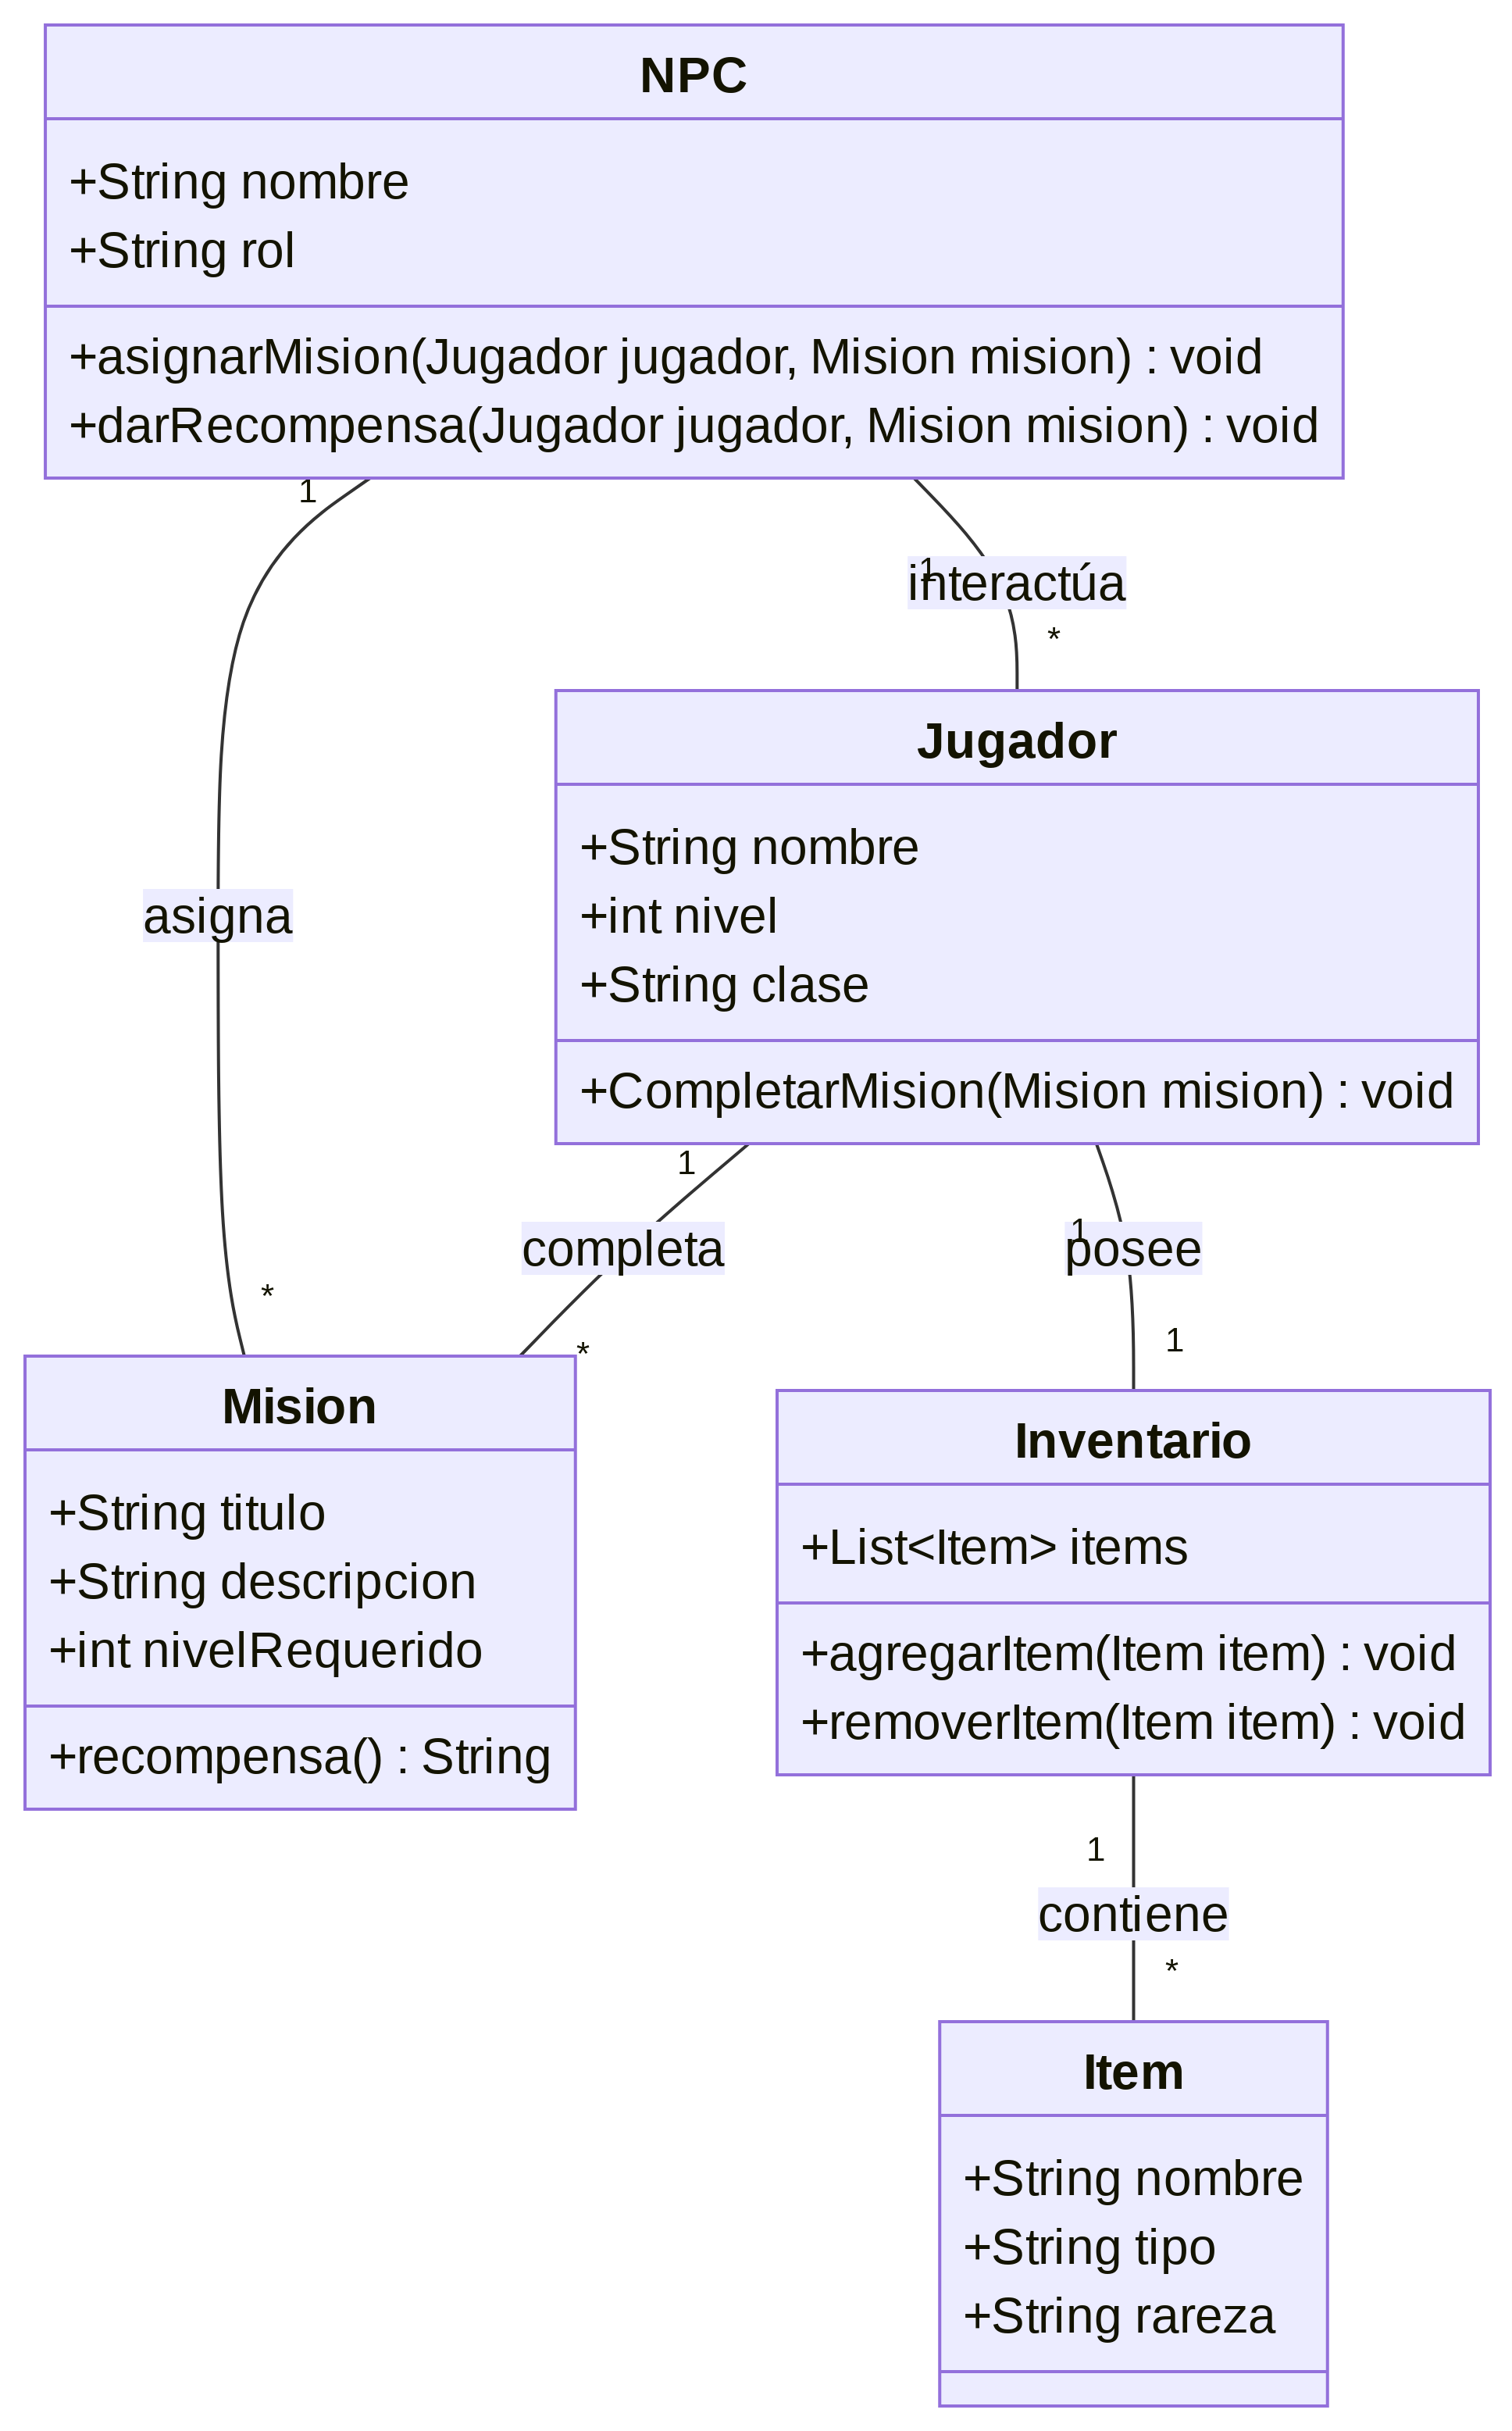
\includegraphics{0A-apéndice1_files/figure-latex/mermaid-figure-1.png}

}

\caption{\label{fig-diagrama}Diagrama de clases.}

\end{figure}%

\chapter{Título del Apéndice 2}\label{ch-apuxe9ndice2}

\section{Otro apéndice: Sección 1}\label{otro-apuxe9ndice-secciuxf3n-1}

\noindent [lipsum {} {]}\{.quarto-shortcode\_\_ data-is-shortcode=``1''
data-raw=``\{\{\textless{} lipsum 2 \textgreater\}\}''\}

\section{Otro apéndice: Sección 2}\label{otro-apuxe9ndice-secciuxf3n-2}





\end{document}
